\chapwithtoc{Introduction} \label{chap:introduction}

% ~~~~~~~~~~~~~~~~~~~~~~~~~~~~~~~~~~~~~~~~~~~~~~~~~~~~~~~~~~~~~~~~~~~~~~~~~~~~~~~~~~~~~~~~~~~~~~~~~~~~~~~~~~~
\section*{Motivation} \label{sec:introduction/motivation}

In modern manufacturing systems, \ac{aps} software is used to schedule production,
manage resources, and analyze complex production data.
This software helps manufacturing planners to schedule production plans
and make important decisions regarding the manufacturing systems.
Modeling and solving such tasks is very difficult, especially in larger manufacturing systems.
The production needs to meet demand while performing optimally with respect to multiple,
often competing, optimization goals.
For humans --- even knowledgeable professionals ---
the set of constraints and conflicting priorities becomes too complex to gain full insight
and consequently decisions can be made without full understanding of the impact.
Conversely, the \ac{aps} software is capable of processing extensive data,
however, not all information can be specified in advance,
nor can all information about the real-world be exactly modeled for the software to consider.
Moreover, the software lacks the intuition of a human production planner,
which undoubtedly plays an important role in making decisions.
This leads to users of the \ac{aps} software to plan production by iteratively
scheduling and fine-tuning settings to obtain an acceptable schedule.

In this thesis, we address the problem of reducing the tardiness
of a selected order in an existing production schedule.
Upon obtaining a schedule constructed to meet all the extensive production demands,
we observe that a particular order is overly tardy with respect to its deadline.
We would like to obtain a modified schedule which reduces the tardiness of that order
while not differing from the original schedule much.
This corresponds to a scenario where, for example, after a discussion with the intended customer,
we need to prioritize the production of the order considered.
However, production has already been scheduled and re-planning it entirely is not acceptable.
Our goal is to find modifications to the schedule,
potentially locally adjusting the settings of the system,
to decrease the tardiness of the target order with minimal impact on the remaining production.

We achieve this by considering manufacturing bottlenecks in the schedule,
related to specific manufacturing constraints.
Our aim is to identify these limiting constraints
and relax them to improve the tardiness of a selected order.
Following the relaxation, we obtain a modified schedule and compare the improvements.
An example of such a modification is illustrated in \cref{fig:schedule-change}.

To model the problem at hand, we use an extension of the \acf{rcpsp}
that introduces time-variant resource capacities.
We develop two different methods to address the problem.
The first method adapts existing approaches from the literature,
which, however, address the problem in simplified scheduling models.
We first need to adapt the approaches to our problem.
The seconds method is developed specifically to address the problem.
This method utilizes relaxations which focus specifically on the target order.
Lastly, we present a set of problem instances designed to model the scheduling problem
and we evaluate the two methods using the presented problem instance set.

\begin{figure}[tb]
    \centering
    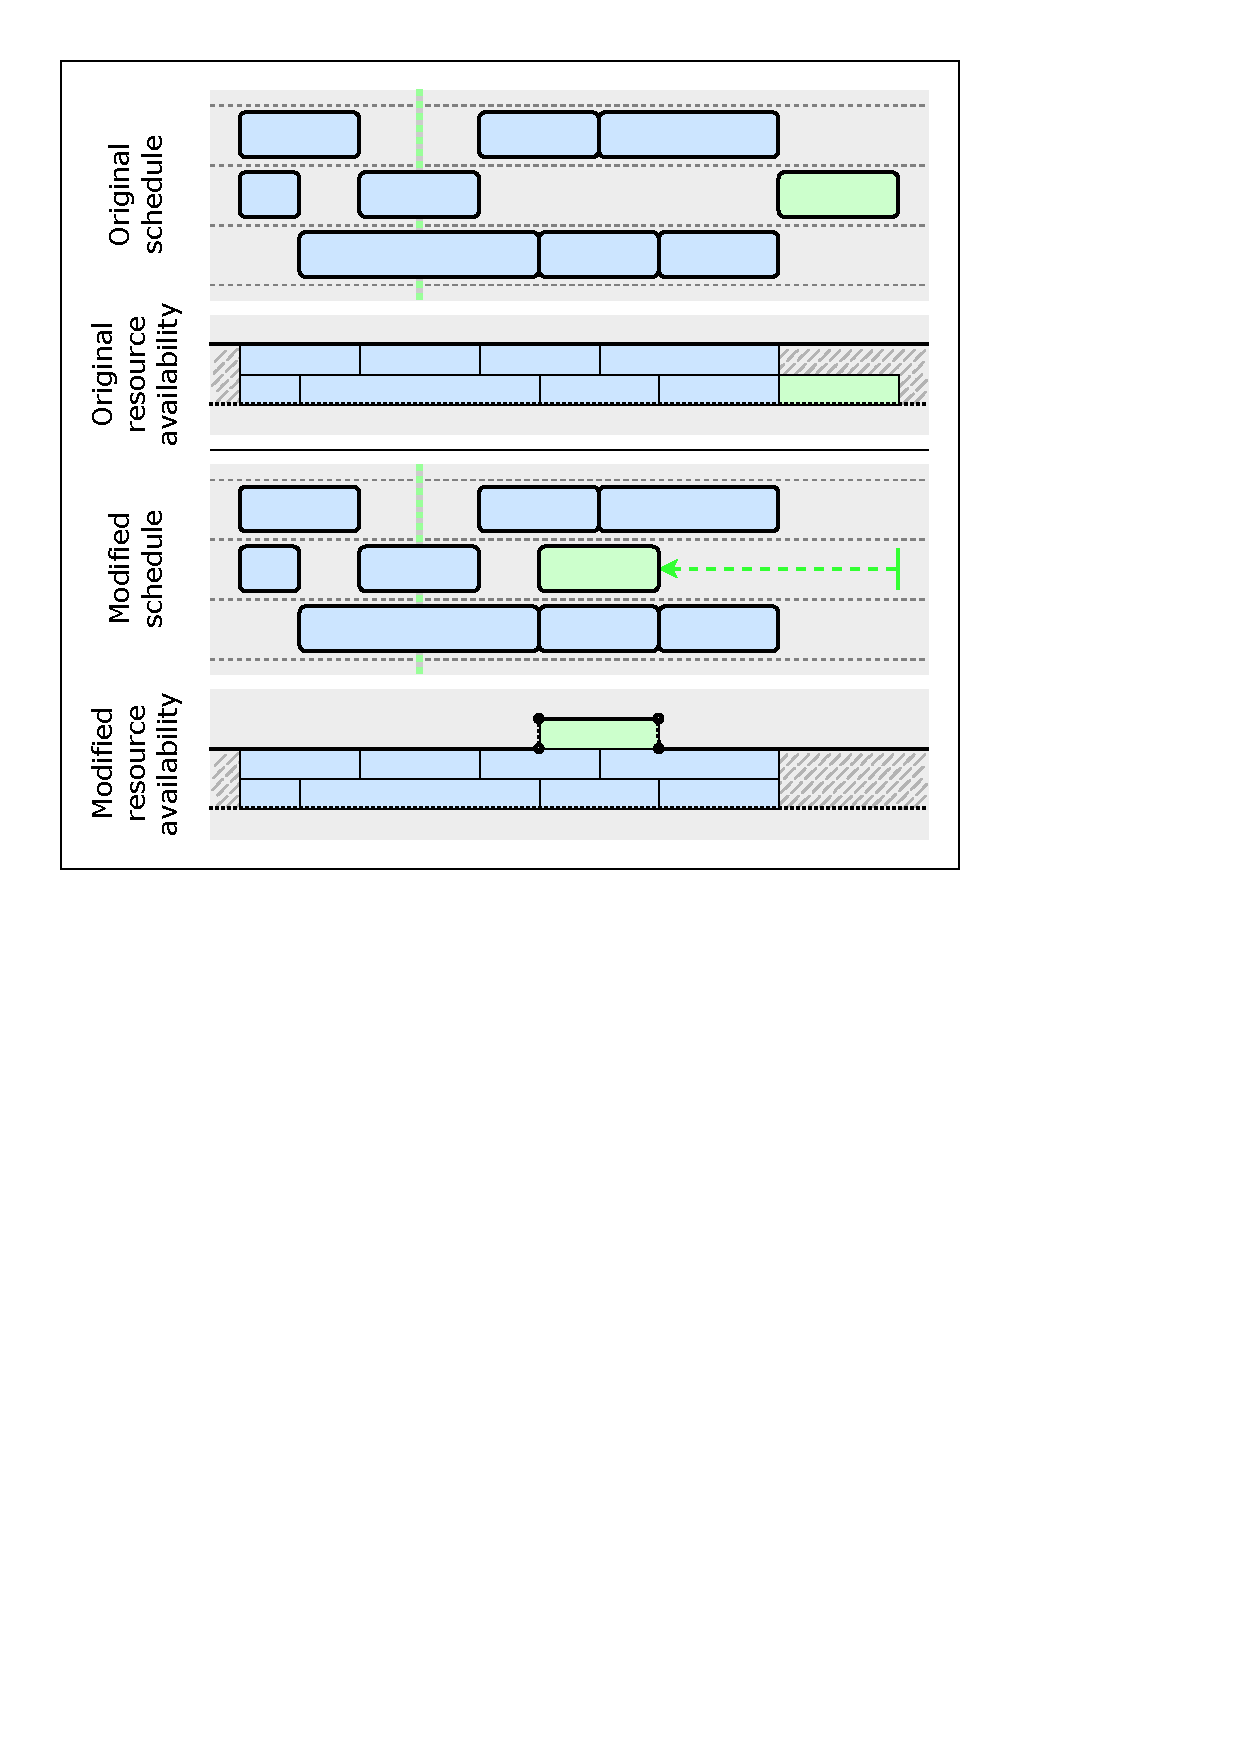
\includegraphics[width=\textwidth]{img/Schedule-Change.pdf}
    \caption{
        Schedule modification example.
        The green highlighted job is overly tardy with respect to its deadline (indicated by the vertical dotted line).
        It could not have been scheduled earlier due to the lack of remaining capacity on the resource.
        The resource capacity is increased within the minimal required time interval
        for the tardy job to be scheduled earlier.
        By temporarily increasing the resource capacity,
        we achieved improvement in the tardiness of the highlighted job,
        as it was possible to schedule it earlier.
        }
    \label{fig:schedule-change}
\end{figure}

% ~~~~~~~~~~~~~~~~~~~~~~~~~~~~~~~~~~~~~~~~~~~~~~~~~~~~~~~~~~~~~~~~~~~~~~~~~~~~~~~~~~~~~~~~~~~~~~~~~~~~~~~~~~~
\section*{Thesis outline} \label{sec:introduction/thesis-outline}

In \cref{chap:problem-statement}, we introduce the problem addressed in this thesis,
followed by a survey of the scheduling literature in \cref{chap:related-works}
aimed to explore various existing approaches to the problem.
In \cref{chap:solution-apporach}, we present our solution approach,
where we design two methods for identifying bottlenecks and relaxing corresponding constraints.
In \cref{chap:numerical-experiments}, we conduct numerical experiments to evaluate the performance
of our proposed methods and discuss achieved results.
In the last chapter, we conclude the thesis by summarizing achieved results
and proposing directions for future work.
